% Definitionen und Befehle
\newcolumntype{Z}[1]{>{\RaggedRight\arraybackslash}p{#1}}%
\newcolumntype{C}[1]{>{\Centering\arraybackslash}p{#1}}%
\newcommand{\talk}[2]%
{%
	& \textbf{#1} \newline \emph{#2}
}%
% Titel -- Redner


\newcommand{\workshop}[3]%
{%
	\workshopbox{#1}{#2}{#3}
}%

\newcommand{\otherevent}[1]%
{%
	& \textbf{#1}
}%

\newcommand{\aulaevent}[2]%
{%
	&
	\multicolumn{3}{c}{
		\textbf{#1} (Aula) \par \emph{#2}
	}
}%

\newcommand{\coffeespace}{\vspace{0.4em}}
\newcommand{\workshopspace}{\vspace{0.5em}\\}

% Farben definieren
\definecolor{commongray}{gray}{.9}
%\vspace{-1.2em}
\renewcommand{\arraystretch}{1.4}


\newpage
\section*{Workshops am Mittwoch}\label{mittwoch-workshops}
	\newsmalltimeslot{10:30 bis 12:00}
	\workshop{52$^\circ§$ North WPS-Workshop}{Benjamin Pross}{1}\workshopspace
	\noindent\workshop{OSM-Daten in QGIS}{Claas Leiner}{2}\workshopspace
	\noindent\workshop{Mapping mit d3}{Mila Frerichs}{3}\workshopspace
	\newsmalltimeslot{15:30 bis 17:00}
	\workshop{Einführung in das Sensor Web}{Simon Jirka}{1}\workshopspace
	\workshop{PostGIS für Einsteiger}{Astrid Emde, Harald Schwenk}{2}\workshopspace
	\workshop{OSM-Daten pflegen und finden mit der Overpass API}{Roland Olbricht}{3}\vfill\newpage
	
\section*{Workshops am Donnerstag}\label{donnerstag-workshops}
	\newsmalltimeslot{09:00 bis 10:30}
	\workshop{Metadaten-Be\-reit\-stellung in INSPIRE-konformen~GDI}{Axel Schaefer}{1}\workshopspace
	\workshop{PostGIS für Einsteiger}{Astrid Emde, Harald Schwenk}{2}\workshopspace
	\workshop{Einführung in die Geodaten-\newline verarbeitung mit Python}{Christian Strobl}{3}\workshopspace
	\newsmalltimeslot{11:15 bis 12:45}
	\workshop{Mapbender3-Workshop}{Astrid Emde, Toni Pignataro}{1}\workshopspace
	\workshop{QGIS-Workshop}{Otto Dassau}{2}\workshopspace
	\workshop{Datenmodel\-lierung mit \mbox{PostgreSQL}/PostGIS für QGIS}{Bernhard Ströbl}{3}\newpage
	
\section*{Workshops am Donnerstag}
	\newsmalltimeslot{14:00 bis 15:30}
	\workshop{MapServer Pro-Tipps}{Jörg Thomsen, Toni Pignataro}{1}\workshopspace
	\workshop{Projektions\-ma\-na\-gement mit QGIS}{Claas Leiner}{2}\workshopspace
	\workshop{Einführungswork\-shop \mbox{OpenLayers}~3}{Marc Jansen}{3}\workshopspace
	\newsmalltimeslot{16:00 bis 17:30}
	\workshop{pgRouting-Workshop}{Daniel Kastl}{1}\workshopspace
	\workshop{QGIS-Server}{Andreas Neumann, Bernhard Ströbl}{2}\workshopspace
	\workshop{Analyse räumlicher Daten mit GRASS GIS~7}{Markus Neteler, Otto Dassau}{3}\newpage

\section*{Workshops am Freitag}\label{freitag-workshops}
	\newsmalltimeslot{09:00 bis 10:30}
	\workshop{Einführung in GeoKettle}{Jens Schaefermeyer}{1}\workshopspace
	\workshop{GeoServer in action}{Daniel Koch, Nils Bühner}{2}\workshopspace
	\workshop{Entwicklung von QGIS-Plugins auf der Basis von PyQt und PyQGIS}{Horst Düster}{3}\workshopspace
	
\label{karte}
%
\ClearWallPaper
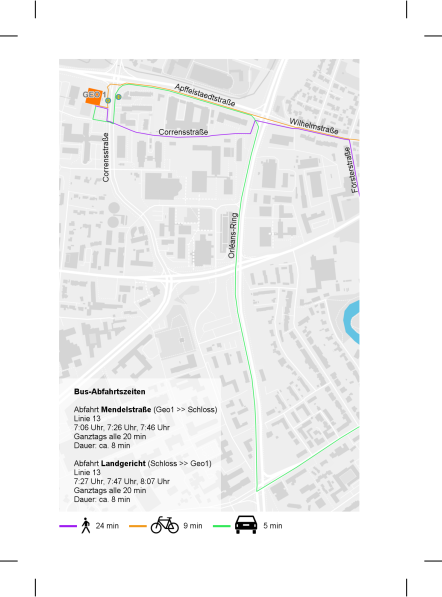
\includepdf{wegkarte-links}
\cropmarkswallpaper
%\ThisCenterWallPaper{1.0}{wegkarte-links}
%\thispagestyle{empty}

\ClearWallPaper
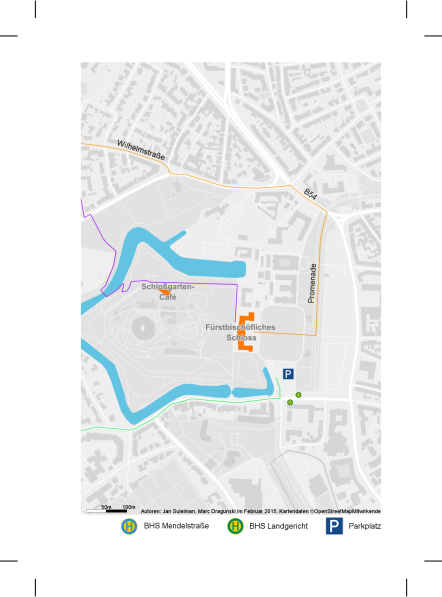
\includepdf{wegkarte-rechts}
\cropmarkswallpaper
\pagebreak

\begin{landscape}	
\ifthispageodd{\ThisCenterWallPaper{1.0}{mittwoch-ungerade}}{\ThisCenterWallPaper{1.0}{mittwoch-gerade}}
\section*{Vorträge am Mittwoch}\label{mittwoch}
\noindent\begin{center}
	\noindent\begin{longtabu}{lZ{4.7cm}Z{4.7cm}}
		& \multicolumn{1}{c}{\cellcolor{hellgruen} S\,1}
		& \multicolumn{1}{c}{\cellcolor{hellorange} Aula} \tabularnewline
		\endhead
		10:30
		\otherevent{Was ist Open-Source? Wie funktioniert das?}\coffeespace
		\talk{}{}
		\coffeespace\tabularnewline
		\rowcolor{commongray}
		12:00 & \multicolumn{2}{c}{%
			\parbox[c]{24pt}{%
				\includegraphics[height=10pt]{cafe}%
			}
			Pause} \tabularnewline
		13:00
		\talk{}{} 
		\talk{Eröffnung}{}
		\tabularnewline
		13:30
		\talk{}{}
		\talk{Nicht zuschauen -- mitmachen!}{Frederik Ramm}
		\coffeespace\tabularnewline
		14:00
		\talk{}{}
		\talk{Softwarewartung für Open-Source -- ein Widerspruch?}{Till Adams}
		\coffeespace\tabularnewline
		\rowcolor{commongray}
		15:00 & \multicolumn{2}{c}{%
			\parbox[c]{24pt}{%
				\includegraphics[height=10pt]{cafe}%
			}
			Kaffeepause} \tabularnewline
	\end{longtabu}	


	\begin{longtabu}{lZ{3cm}Z{3cm}Z{3cm}}
		& \multicolumn{1}{c}{\cellcolor{hellgruen} S\,1}
		& \multicolumn{1}{c}{\cellcolor{hellgelb} S\,2}
		& \multicolumn{1}{c}{\cellcolor{geoblau} S\,10} \tabularnewline
		\endhead
		15:30
		\talk{Welches Münster meinen sie?}{Marc Tobias Metten}
		\talk{Umsetzung der INSPIRE-Richtlinie}{Jürgen Weichand}
		\talk{Neues von QGIS 2.8}{Horst Düster}
		\coffeespace\tabularnewline
		16:00
		\talk{Offene Geodaten -- Lage von Orten im Vergleich}{Thomas Brinkhoff}\coffeespace
		\talk{GeoPortal.rlp}{Armin Retterath}
		\talk{QGIS-Plugins}{Pirmin Kalberer}
		\coffeespace\tabularnewline
		16:30
		\talk{OSM-Tagging in Wikidata}{Tim Alder}
		\talk{Geonetzwerk metropoleRuhr}{David Arndt}
		\talk{QGIS Print Com\-poser und Atlas-Seriendruck}{Andreas Neumann}
		\coffeespace\tabularnewline
		17:00
		\talk{Ein GeoWiki auf OSM-Basis}{Klaus Stein}
		\talk{Spatial Index von Solr}{Tim Balschmiter\vspace{0.5em}}
		\talk{QField for QGIS}{Marco Bernasocchi}
		\coffeespace\coffeespace\tabularnewline
		\rowcolor{commongray}
		17:30 &
		\multicolumn{3}{c}{%
			\textbf{Anwendertreffen/BoFs} (siehe Seite \pageref{bof-mittwoch})}
		\tabularnewline
	\end{longtabu}	
	\ThisCenterWallPaper{1.0}{mittwoch-ungerade}
	\enlargethispage{0.5em}
\end{center}
\end{landscape}

\renewcommand{\arraystretch}{1}